\begin{frame}{Flujo Laminar y Turbulento}
\justifying
El flujo laminar y turbulento son aspectos fluídicos de un flujo viscoso. En un flujo laminar las líneas de corriente son paralelas y en el caso de una tubería circular estas son cilíndros concéntricos alrededor de la línea de flujo central.
La transición de laminar a turbulento ocurre generalmente debido a los cambios de velocidad o geometría.
\begin{figure}[H]
\centering
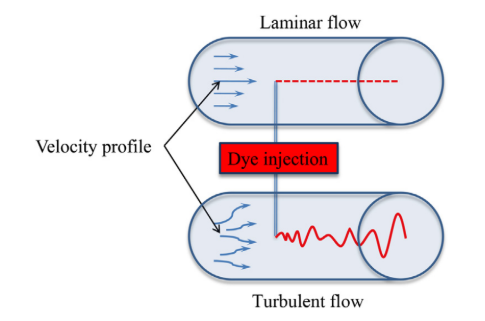
\includegraphics[scale=0.4]{Section_Files/S2-imagenes-Manuel/02.png}
\caption{Tinte sobre una corriente de flujo Newtoneano para demostrar el fluido laminar y turbulento.}
\end{figure}
{\tiny Biofluid Mechanics Aplications por Ali Ostadfar, pag. 20}
\end{frame}

\begin{frame}{Perfil de velocidad}
\justifying
Es un diagrama de vectores de velocidad de una corriente de fluido como una función de la distancia perpendicular a la dirección del flujo.
\begin{figure}[H]
\centering
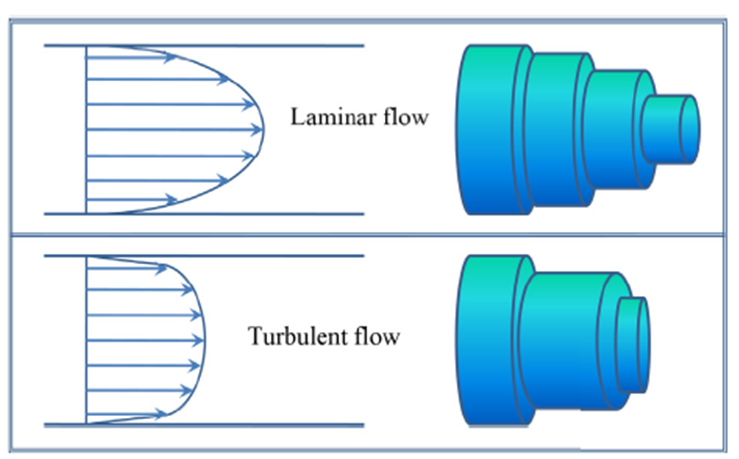
\includegraphics[scale=0.4]{Section_Files/S2-imagenes-Manuel/03.png}
\caption{Esquema de perfil de velocidad para un flujo laminar y turbulento.}
\end{figure}
{\tiny Biofluid Mechanics Aplications por Ali Ostadfar, pag. 20}
\end{frame}

\begin{frame}{Flujo laminar}
\justifying
Para un flujo viscoso a través de un canal circular, el perfil de velocidad axial esta dado por:
\begin{figure}[H]
\centering
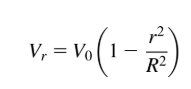
\includegraphics[scale=0.4]{Section_Files/S2-imagenes-Manuel/04.png}
\end{figure}
\begin{figure}[H]
\centering
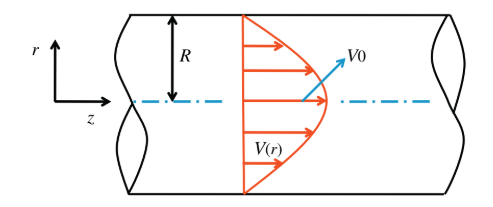
\includegraphics[scale=0.3]{Section_Files/S2-imagenes-Manuel/05.png}
\end{figure}
{\tiny Biofluid Mechanics Aplications por Ali Ostadfar, pag. 21}
\end{frame}

\begin{frame}{Flujo turbulento}
\justifying
\begin{itemize}
\item El flujo varía constantemente y este tiene un comportamiento caótico.
\item El esfuerzo cortante entre capas aumenta.
\item El número de Reynolds ayuda a evaluar si el fluido es laminar o turbulento.
\end{itemize}

\begin{figure}[H]
\centering
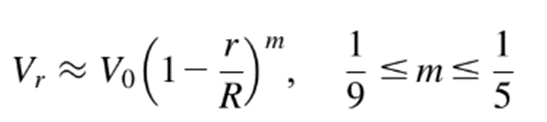
\includegraphics[scale=0.25]{Section_Files/S2-imagenes-Manuel/06.png}
\caption{Where Vr is axial velocity as a function of radius. Vo is maximun velocity at the certerline, r is radial distance from the centerline and R is radius of the channel.}
\end{figure}
\begin{figure}[H]
\centering
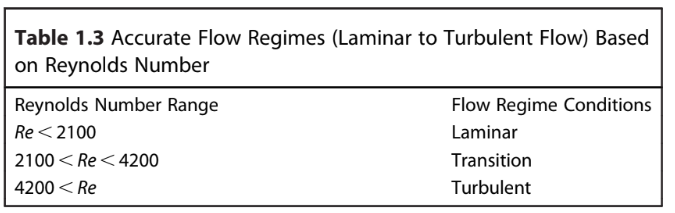
\includegraphics[scale=0.3]{Section_Files/S2-imagenes-Manuel/08.png}
\end{figure}
{\tiny Biofluid Mechanics Aplications por Ali Ostadfar, pag. 21}
\end{frame}

\begin{frame}{Flujo turbulento - Ejercicio}
\justifying
\begin{figure}[H]
\centering
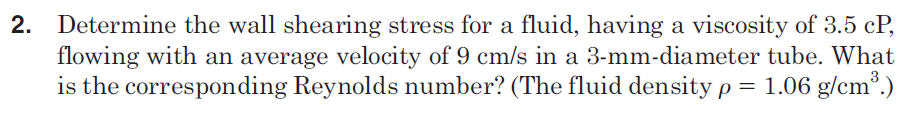
\includegraphics[scale=0.4]{Section_Files/S2-imagenes-Manuel/09.png}
\end{figure}
{\tiny Biofluid Mechanics Aplications por Ali Ostadfar, pag. 31}
\end{frame}

\begin{frame}{Flujo turbulento - Ejercicio}
\justifying
\begin{figure}[H]
\centering
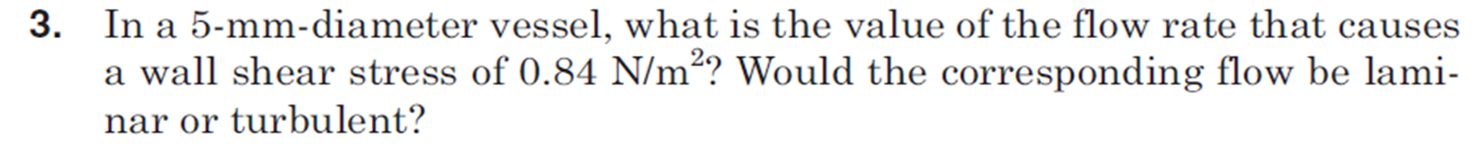
\includegraphics[scale=0.4]{Section_Files/S2-imagenes-Manuel/10.png}
\end{figure}
{\tiny Biofluid Mechanics Aplications por Ali Ostadfar, pag. 31}
\end{frame}

\begin{frame}{Flujo turbulento - Ejercicio}
\justifying
\begin{figure}[H]
\centering
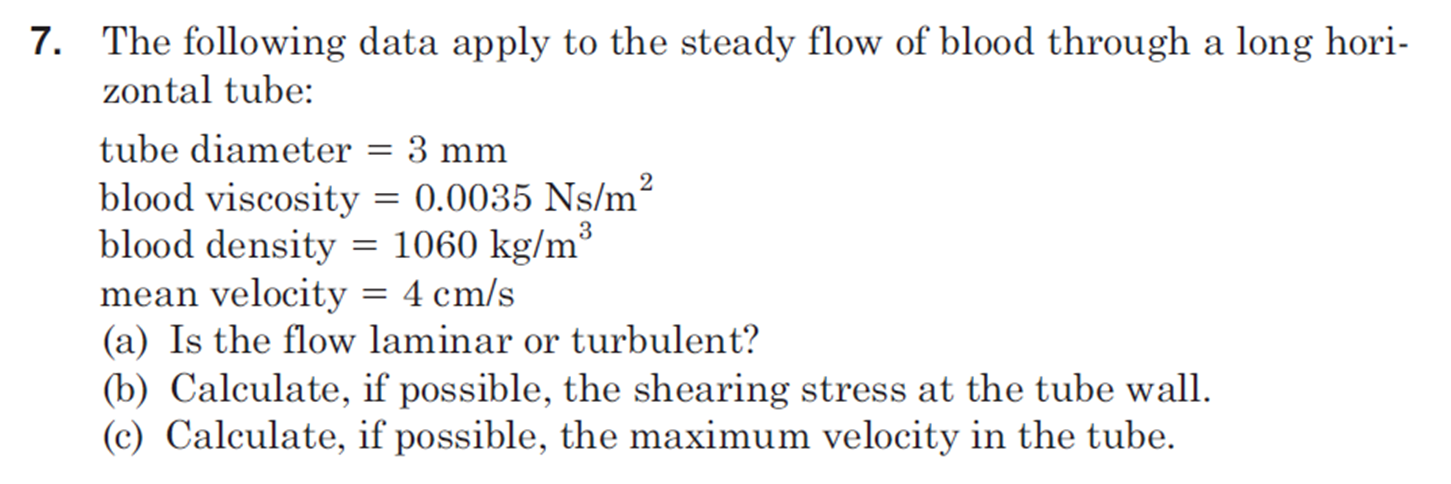
\includegraphics[scale=0.4]{Section_Files/S2-imagenes-Manuel/11.png}
\end{figure}
{\tiny Biofluid Mechanics Aplications por Ali Ostadfar, pag. 32}
\end{frame}

\begin{frame}{Flujo turbulento - Ejercicio}
\justifying
\begin{figure}[H]
\centering
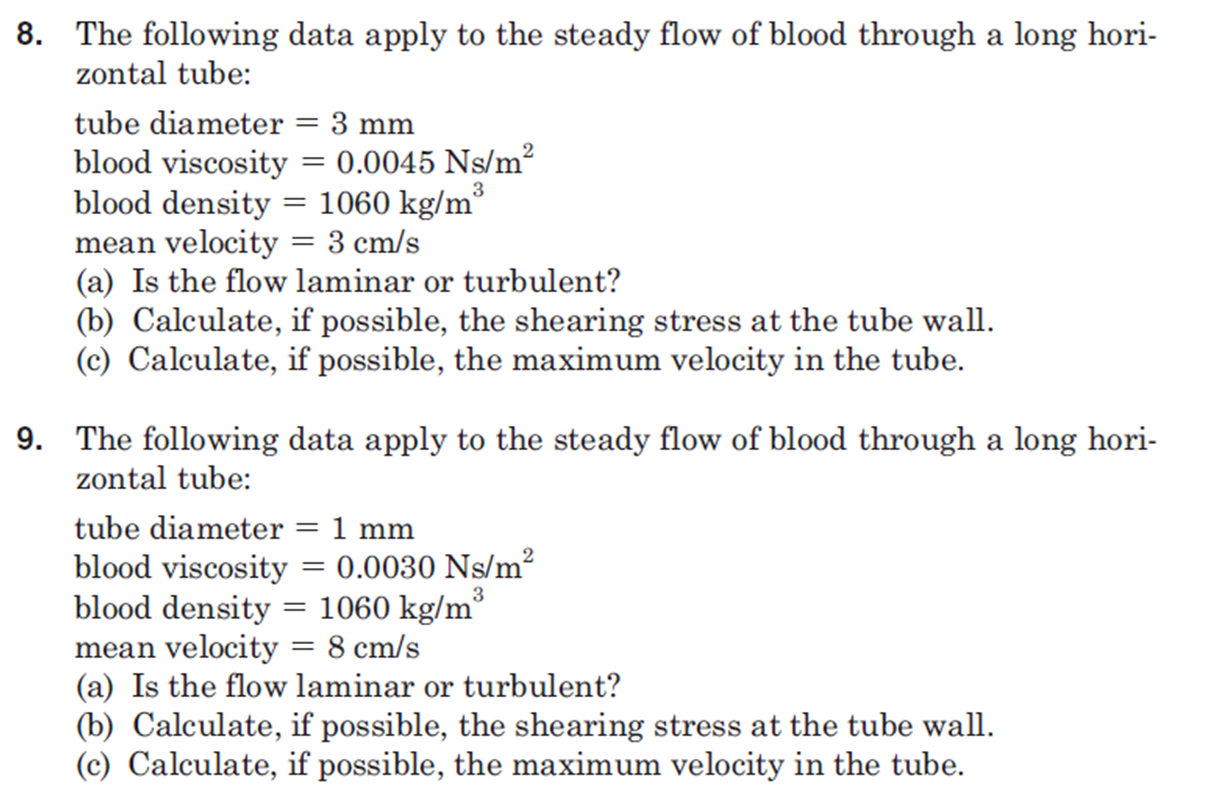
\includegraphics[scale=0.4]{Section_Files/S2-imagenes-Manuel/12.png}
\end{figure}
{\tiny Biofluid Mechanics Aplications por Ali Ostadfar, pag. 32}
\end{frame}

\begin{frame}{Condiciones de borde y no deslizamiento}
\justifying
Las ecuaciones tienen un rol importante en las aplicaciones físicas. Las ecuaciones que gobiernan las características físicas, como presión y velocidad, están definidas por ecuaciones diferenciales parciales. Para calcular estas ecuaciones es necesario conocer datos iniciales, como el camp'o de velocidades en el campo de los fluidos. Estos datos son conocidos como condiciones de contorno o borde.
\begin{figure}[H]
\centering
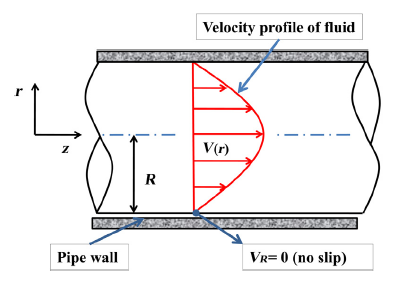
\includegraphics[scale=0.4]{Section_Files/S2-imagenes-Manuel/13.png}
\caption{Esquema de condición de contorno de no deslizamiento. La velocidad tangencial en el punto entre la interface líquido-sólido de la pared de la tubería es igual a cero ($V(R)=0m/s)$.}
\end{figure}
{\tiny Biofluid Mechanics Aplications por Ali Ostadfar, pag. 32}
\end{frame}